% Options for packages loaded elsewhere
\PassOptionsToPackage{unicode}{hyperref}
\PassOptionsToPackage{hyphens}{url}
%
\documentclass[
]{book}
\usepackage{amsmath,amssymb}
\usepackage{lmodern}
\usepackage{ifxetex,ifluatex}
\ifnum 0\ifxetex 1\fi\ifluatex 1\fi=0 % if pdftex
  \usepackage[T1]{fontenc}
  \usepackage[utf8]{inputenc}
  \usepackage{textcomp} % provide euro and other symbols
\else % if luatex or xetex
  \usepackage{unicode-math}
  \defaultfontfeatures{Scale=MatchLowercase}
  \defaultfontfeatures[\rmfamily]{Ligatures=TeX,Scale=1}
\fi
% Use upquote if available, for straight quotes in verbatim environments
\IfFileExists{upquote.sty}{\usepackage{upquote}}{}
\IfFileExists{microtype.sty}{% use microtype if available
  \usepackage[]{microtype}
  \UseMicrotypeSet[protrusion]{basicmath} % disable protrusion for tt fonts
}{}
\makeatletter
\@ifundefined{KOMAClassName}{% if non-KOMA class
  \IfFileExists{parskip.sty}{%
    \usepackage{parskip}
  }{% else
    \setlength{\parindent}{0pt}
    \setlength{\parskip}{6pt plus 2pt minus 1pt}}
}{% if KOMA class
  \KOMAoptions{parskip=half}}
\makeatother
\usepackage{xcolor}
\IfFileExists{xurl.sty}{\usepackage{xurl}}{} % add URL line breaks if available
\IfFileExists{bookmark.sty}{\usepackage{bookmark}}{\usepackage{hyperref}}
\hypersetup{
  pdftitle={ShinyDataSHIELD User's Guide},
  pdfauthor={Escribà Montagut, Xavier; González, Juan R.},
  hidelinks,
  pdfcreator={LaTeX via pandoc}}
\urlstyle{same} % disable monospaced font for URLs
\usepackage{color}
\usepackage{fancyvrb}
\newcommand{\VerbBar}{|}
\newcommand{\VERB}{\Verb[commandchars=\\\{\}]}
\DefineVerbatimEnvironment{Highlighting}{Verbatim}{commandchars=\\\{\}}
% Add ',fontsize=\small' for more characters per line
\usepackage{framed}
\definecolor{shadecolor}{RGB}{248,248,248}
\newenvironment{Shaded}{\begin{snugshade}}{\end{snugshade}}
\newcommand{\AlertTok}[1]{\textcolor[rgb]{0.94,0.16,0.16}{#1}}
\newcommand{\AnnotationTok}[1]{\textcolor[rgb]{0.56,0.35,0.01}{\textbf{\textit{#1}}}}
\newcommand{\AttributeTok}[1]{\textcolor[rgb]{0.77,0.63,0.00}{#1}}
\newcommand{\BaseNTok}[1]{\textcolor[rgb]{0.00,0.00,0.81}{#1}}
\newcommand{\BuiltInTok}[1]{#1}
\newcommand{\CharTok}[1]{\textcolor[rgb]{0.31,0.60,0.02}{#1}}
\newcommand{\CommentTok}[1]{\textcolor[rgb]{0.56,0.35,0.01}{\textit{#1}}}
\newcommand{\CommentVarTok}[1]{\textcolor[rgb]{0.56,0.35,0.01}{\textbf{\textit{#1}}}}
\newcommand{\ConstantTok}[1]{\textcolor[rgb]{0.00,0.00,0.00}{#1}}
\newcommand{\ControlFlowTok}[1]{\textcolor[rgb]{0.13,0.29,0.53}{\textbf{#1}}}
\newcommand{\DataTypeTok}[1]{\textcolor[rgb]{0.13,0.29,0.53}{#1}}
\newcommand{\DecValTok}[1]{\textcolor[rgb]{0.00,0.00,0.81}{#1}}
\newcommand{\DocumentationTok}[1]{\textcolor[rgb]{0.56,0.35,0.01}{\textbf{\textit{#1}}}}
\newcommand{\ErrorTok}[1]{\textcolor[rgb]{0.64,0.00,0.00}{\textbf{#1}}}
\newcommand{\ExtensionTok}[1]{#1}
\newcommand{\FloatTok}[1]{\textcolor[rgb]{0.00,0.00,0.81}{#1}}
\newcommand{\FunctionTok}[1]{\textcolor[rgb]{0.00,0.00,0.00}{#1}}
\newcommand{\ImportTok}[1]{#1}
\newcommand{\InformationTok}[1]{\textcolor[rgb]{0.56,0.35,0.01}{\textbf{\textit{#1}}}}
\newcommand{\KeywordTok}[1]{\textcolor[rgb]{0.13,0.29,0.53}{\textbf{#1}}}
\newcommand{\NormalTok}[1]{#1}
\newcommand{\OperatorTok}[1]{\textcolor[rgb]{0.81,0.36,0.00}{\textbf{#1}}}
\newcommand{\OtherTok}[1]{\textcolor[rgb]{0.56,0.35,0.01}{#1}}
\newcommand{\PreprocessorTok}[1]{\textcolor[rgb]{0.56,0.35,0.01}{\textit{#1}}}
\newcommand{\RegionMarkerTok}[1]{#1}
\newcommand{\SpecialCharTok}[1]{\textcolor[rgb]{0.00,0.00,0.00}{#1}}
\newcommand{\SpecialStringTok}[1]{\textcolor[rgb]{0.31,0.60,0.02}{#1}}
\newcommand{\StringTok}[1]{\textcolor[rgb]{0.31,0.60,0.02}{#1}}
\newcommand{\VariableTok}[1]{\textcolor[rgb]{0.00,0.00,0.00}{#1}}
\newcommand{\VerbatimStringTok}[1]{\textcolor[rgb]{0.31,0.60,0.02}{#1}}
\newcommand{\WarningTok}[1]{\textcolor[rgb]{0.56,0.35,0.01}{\textbf{\textit{#1}}}}
\usepackage{longtable,booktabs,array}
\usepackage{calc} % for calculating minipage widths
% Correct order of tables after \paragraph or \subparagraph
\usepackage{etoolbox}
\makeatletter
\patchcmd\longtable{\par}{\if@noskipsec\mbox{}\fi\par}{}{}
\makeatother
% Allow footnotes in longtable head/foot
\IfFileExists{footnotehyper.sty}{\usepackage{footnotehyper}}{\usepackage{footnote}}
\makesavenoteenv{longtable}
\usepackage{graphicx}
\makeatletter
\def\maxwidth{\ifdim\Gin@nat@width>\linewidth\linewidth\else\Gin@nat@width\fi}
\def\maxheight{\ifdim\Gin@nat@height>\textheight\textheight\else\Gin@nat@height\fi}
\makeatother
% Scale images if necessary, so that they will not overflow the page
% margins by default, and it is still possible to overwrite the defaults
% using explicit options in \includegraphics[width, height, ...]{}
\setkeys{Gin}{width=\maxwidth,height=\maxheight,keepaspectratio}
% Set default figure placement to htbp
\makeatletter
\def\fps@figure{htbp}
\makeatother
\setlength{\emergencystretch}{3em} % prevent overfull lines
\providecommand{\tightlist}{%
  \setlength{\itemsep}{0pt}\setlength{\parskip}{0pt}}
\setcounter{secnumdepth}{5}
\usepackage{booktabs}
\ifluatex
  \usepackage{selnolig}  % disable illegal ligatures
\fi
\usepackage[]{natbib}
\bibliographystyle{apalike}

\title{ShinyDataSHIELD User's Guide}
\author{Escribà Montagut, Xavier; González, Juan R.}
\date{2022-01-17}

\begin{document}
\maketitle

{
\setcounter{tocdepth}{1}
\tableofcontents
}
\hypertarget{overview}{%
\chapter{Overview}\label{overview}}


\includegraphics[width=0.5\textwidth,height=\textheight]{fig/ds_logo.png}

ShinyDataSHIELD is a non-disclosive data analysis toolbox powered by DataSHIELD with the following features:

\begin{itemize}
\tightlist
\item
  Descriptive statistics: Summary, scatter plots, histograms and heatmaps of table variables.
\item
  Statistic models: GLM and GLMer model fittings
\item
  Omic analysis: GWAS, LIMMA, \ldots{} using different types of resources (VCF files, PLINK, RSE, eSets)
\end{itemize}

The features available on ShinyDataSHIELD are powered by different packages of the DataSHIELD project (dsBaseClient and dsOmicsClient), it uses them in a seamless way so the final user of ShinyDataSHIELD can perform all the included studies without writing a single line of code and get all the resulting figures and tables by the click of a button.

a

\hypertarget{Omic}{%
\chapter{Omic data analysis: types of implemented analyses}\label{Omic}}

The Figure \ref{fig:opalOmic} describes the different types of 'omic association analyses that can be performed using DataSHIELD client functions implemented in the \emph{\href{https://github.com/isglobal-brge/dsOmicsClient}{dsOmicsClient}} package. Basically, data ('omic and phenotypes/covariates) can be stored in different sites (http, ssh, AWS S3, local, \ldots) and are managed with Opal through the \emph{\href{https://github.com/obiba/resourcer}{resourcer}} package and their extensions implemented in \emph{\href{https://github.com/isglobal-brge/dsOmics}{dsOmics}}.

\begin{figure}

{\centering 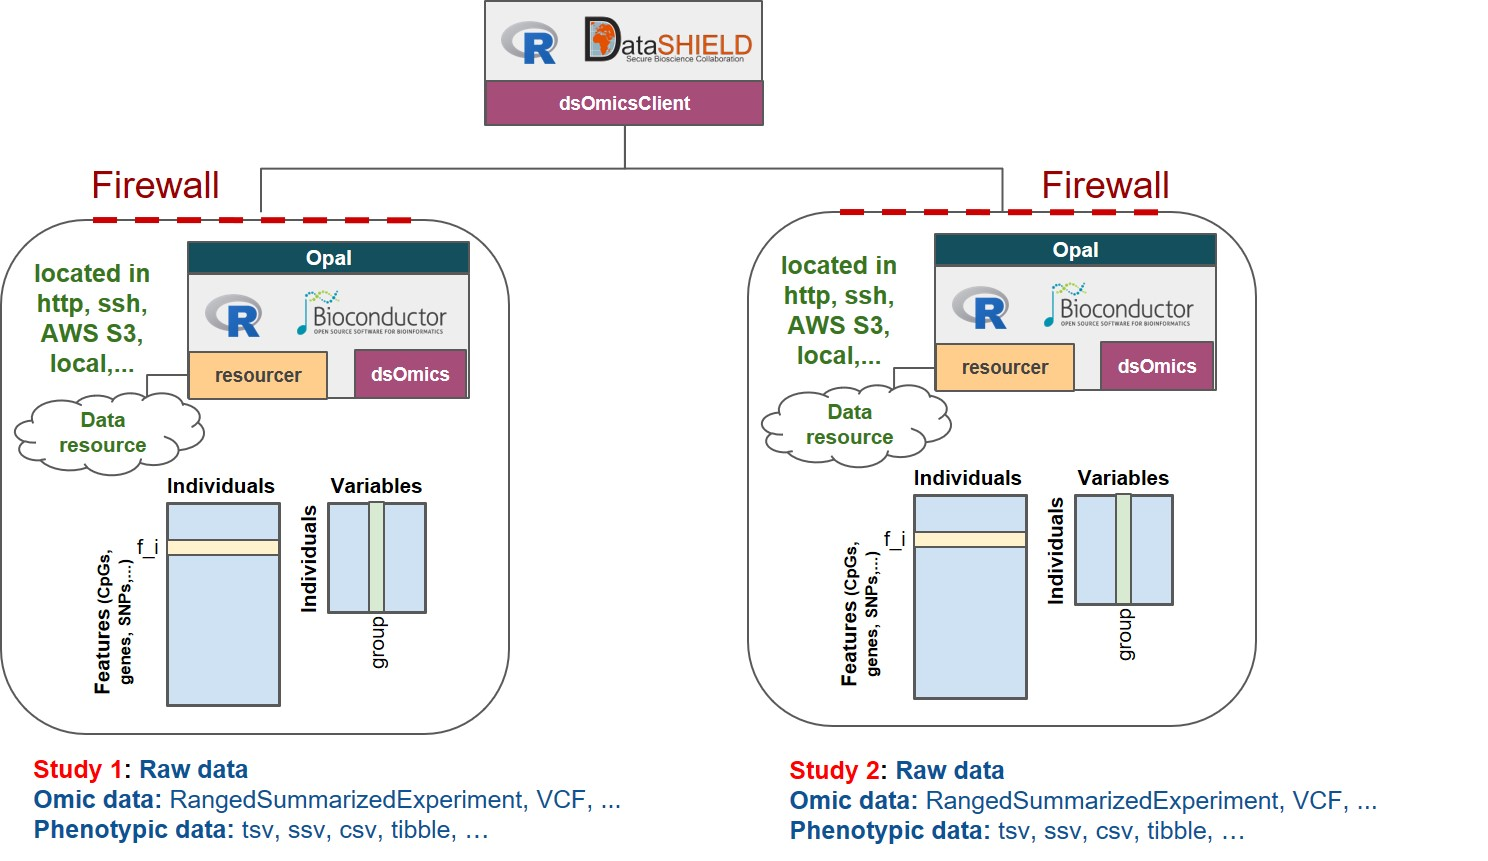
\includegraphics[width=20.67in]{fig/dsOmics_A} 

}

\caption{Non-disclosive omic data analysis with DataSHIELD and Bioconductor. The figure illustrates how the `resourcer` package is used to get access to omic data through the Opal servers. Then DataSHIELD is used in the client side to perform non-disclosive data analyses.}\label{fig:opalOmic}
\end{figure}

Then, \texttt{dsOmicsClient} package allows different types of analyses: pooled and meta-analysis. Both methods are based on fitting different Generalized Linear Models (GLMs) for each feature when assesing association between 'omic data and the phenotype/trait/condition of interest. Of course, non-disclosive 'omic data analysis from a single study can also be performed.

The \textbf{pooled approach} (Figure \ref{fig:omicAnal1}) is recommended when the user wants to analyze 'omic data from different sources and obtain results as if the data were located in a single computer. It should be noted that this can be very time consuming when analyzing multiple features since it calls a base function in DataSHIELD (\texttt{ds.glm}) repeatedly. It also cannot be recommended when data are not properly harmonized (e.g.~gene expression normalized using different methods, GWAS data having different platforms, \ldots). Furthermore when it is necesary to remove unwanted variability (for transcriptomic and epigenomica analysis) or control for population stratification (for GWAS analysis), this approach cannot be used since we need to develop methods to compute surrogate variables (to remove unwanted variability) or PCAs (to to address population stratification) in a non-disclosive way.

The \textbf{meta-analysis approach} Figure \ref{fig:omicAnal2} overcomes the limitations raised when performing pooled analyses. First, the computation issue is addressed by using scalable and fast methods to perform data analysis at whole-genome level at each location The transcriptomic and epigenomic data analyses make use of the widely used \emph{\href{https://bioconductor.org/packages/3.12/limma}{limma}} package that uses \texttt{ExpressionSet} or \texttt{RangedSummarizedExperiment} Bioc infrastructures to deal with 'omic and phenotypic (e.g covariates). The genomic data are analyzed using \emph{\href{https://bioconductor.org/packages/3.12/GWASTools}{GWASTools}} and \emph{\href{https://bioconductor.org/packages/3.12/GENESIS}{GENESIS}} that are designed to perform quality control (QC) and GWAS using GDS infrastructure.

Next, we describe how both approaches are implemented:

\begin{itemize}
\tightlist
\item
  \textbf{Pooled approach:} Figure \ref{fig:omicAnal1} illustrate how this analysis is performed. This corresponds to generalized linear models (glm) on data from single or multiple sources. It makes use of \texttt{ds.glm()} function which is a DataSHIELD function that uses an approach that is mathematically equivalent to placing all individual-level data froma all sources in one central warehouse and analysing those data using the conventional \texttt{glm()} function in R. The user can select one (or multiple) features (i.e., genes, transcripts, CpGs, SNPs, \ldots)
\end{itemize}

\begin{figure}

{\centering 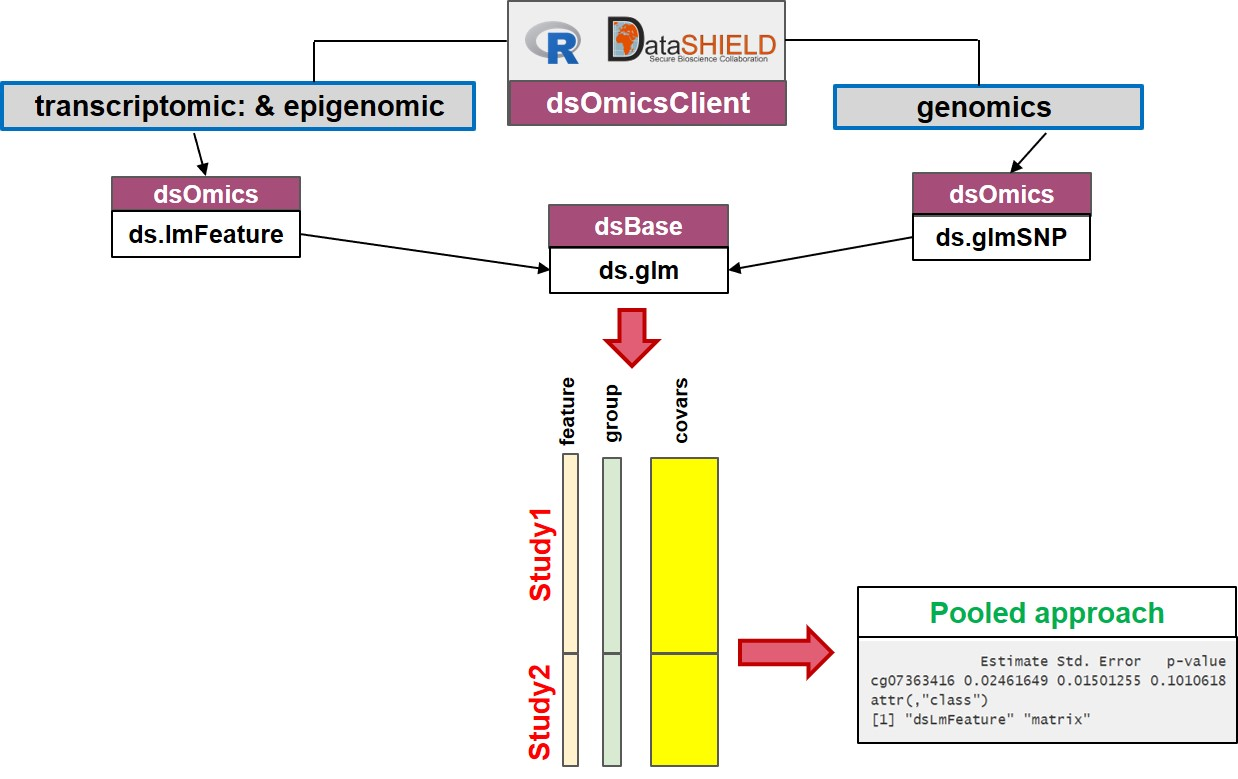
\includegraphics[width=17.19in]{fig/dsOmics_B} 

}

\caption{Non-disclosive omic data analysis with DataSHIELD and Bioconductor. The figure illustrates how to perform single pooled omic data analysis. The analyses are performed by using a generalized linear model (glm) on data from one or multiple sources. It makes use of `ds.glm()`, a DataSHIELD function, that uses an approach that is mathematically equivalent to placing all individual-level data from all sources in one central warehouse and analysing those data using the conventional `glm()` function in R.}\label{fig:omicAnal1}
\end{figure}

\begin{itemize}
\tightlist
\item
  \textbf{Meta-analysis:} Figure \ref{fig:omicAnal2} illustrate how this analysis is performed. This corresponds to performing a genome-wide analysis at each location using functions that are specifically design for that purpose and that are scalable. Then the results from each location can be meta-analyzed using methods that meta-analyze either effect sizes or p-values.
\end{itemize}

\begin{figure}

{\centering 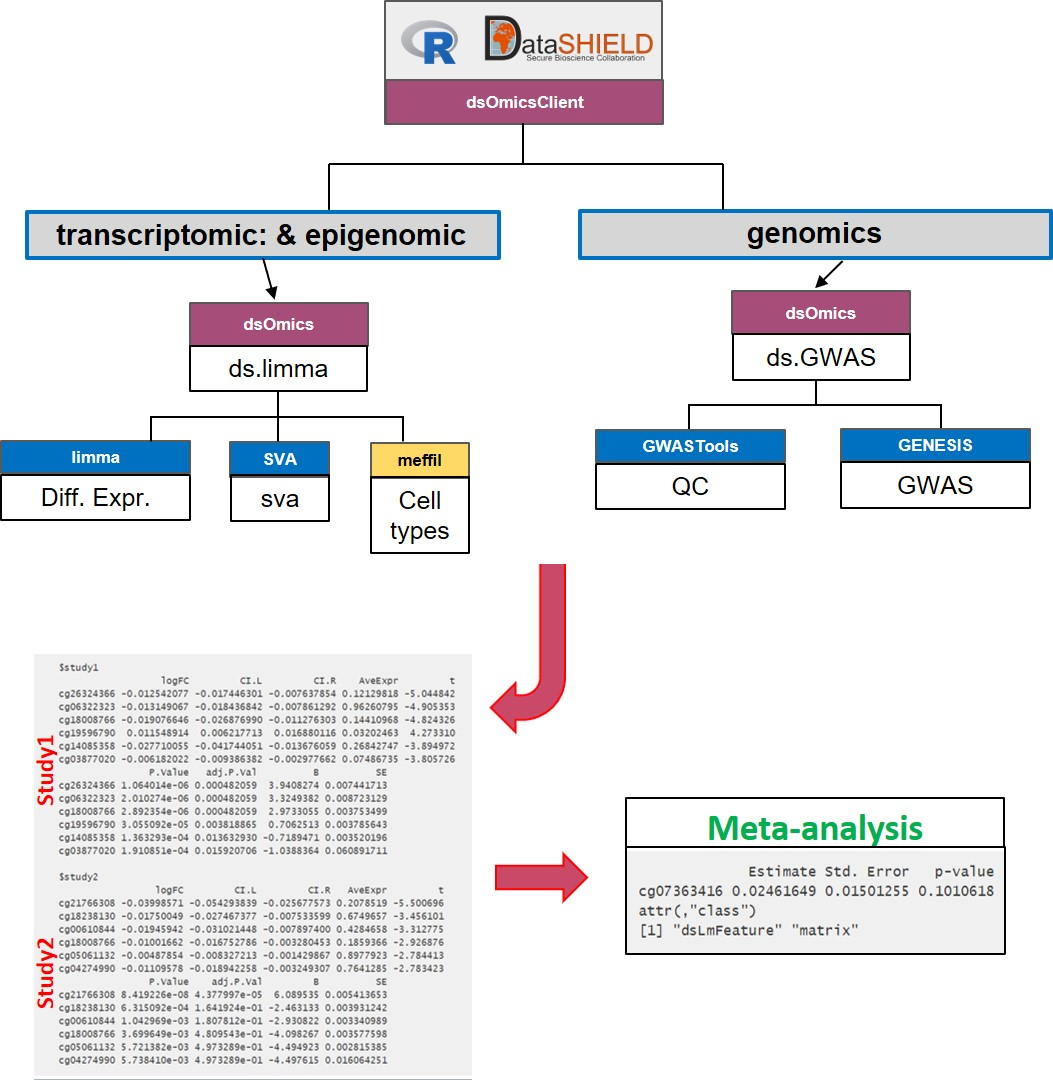
\includegraphics[width=14.62in]{fig/dsOmics_C} 

}

\caption{Non-disclosive omic data analysis with DataSHIELD and Bioconductor. The figure illustrates how to perform anlyses at genome-wide level from one or multiple sources. It runs standard Bioconductor functions at each server independently to speed up the analyses and in the case of having multiple sources, results can be meta-analyzed uning standar R functions.}\label{fig:omicAnal2}
\end{figure}

\hypertarget{differential-gene-expression-dge-analysis}{%
\chapter{Differential gene expression (DGE) analysis}\label{differential-gene-expression-dge-analysis}}

Let us illustrate how to perform transcriptomic data analysis using data from \href{https://www.cancer.gov/about-nci/organization/ccg/research/structural-genomics/tcga}{TCGA project}. We have uploaded to the opal server a resource called \texttt{tcga\_liver} whose URL is \url{http://duffel.rail.bio/recount/TCGA/rse_gene_liver.Rdata} which is available through the \href{https://jhubiostatistics.shinyapps.io/recount/}{recount project}. This resource contains the \texttt{RangeSummarizedExperiment} with the RNAseq profiling of liver cancer data from TCGA. Next, we illustrate how a differential expression analysis to compare RNAseq profiling of women vs men (variable \texttt{gdc\_cases.demographic.gender}). The DGE analysis is normally performed using \emph{\href{https://bioconductor.org/packages/3.12/limma}{limma}} package. In that case, as we are analyzing RNA-seq data, \texttt{limma\ +\ voom} method will be required.

Let us start by creating the connection to the opal server:

\begin{Shaded}
\begin{Highlighting}[]
\NormalTok{builder }\OtherTok{\textless{}{-}} \FunctionTok{newDSLoginBuilder}\NormalTok{()}
\NormalTok{builder}\SpecialCharTok{$}\FunctionTok{append}\NormalTok{(}\AttributeTok{server =} \StringTok{"study1"}\NormalTok{, }\AttributeTok{url =} \StringTok{"https://opal{-}demo.obiba.org"}\NormalTok{, }
               \AttributeTok{user =} \StringTok{"dsuser"}\NormalTok{, }\AttributeTok{password =} \StringTok{"P@ssw0rd"}\NormalTok{, }
               \AttributeTok{resource =} \StringTok{"RSRC.tcga\_liver"}\NormalTok{, }\AttributeTok{profile =} \StringTok{"omics"}\NormalTok{)}

\NormalTok{logindata }\OtherTok{\textless{}{-}}\NormalTok{ builder}\SpecialCharTok{$}\FunctionTok{build}\NormalTok{()}

\NormalTok{conns }\OtherTok{\textless{}{-}} \FunctionTok{datashield.login}\NormalTok{(}\AttributeTok{logins =}\NormalTok{ logindata, }\AttributeTok{assign =} \ConstantTok{TRUE}\NormalTok{, }
                          \AttributeTok{symbol =} \StringTok{"res"}\NormalTok{)}
\end{Highlighting}
\end{Shaded}

\begin{verbatim}
## 
## Logging into the collaborating servers
\end{verbatim}

\begin{verbatim}
## 
## Assigning resource data...
\end{verbatim}

Then, let us coerce the resource to a \texttt{RangedSummarizedExperiment} which is the type of object that is available in the \href{https://jhubiostatistics.shinyapps.io/recount/}{recount project}.

\begin{Shaded}
\begin{Highlighting}[]
\FunctionTok{datashield.assign.expr}\NormalTok{(conns, }\AttributeTok{symbol =} \StringTok{"rse"}\NormalTok{, }
                       \AttributeTok{expr =} \FunctionTok{quote}\NormalTok{(}\FunctionTok{as.resource.object}\NormalTok{(res)))}
\FunctionTok{ds.class}\NormalTok{(}\StringTok{"rse"}\NormalTok{)}
\end{Highlighting}
\end{Shaded}

\begin{verbatim}
## $study1
## [1] "RangedSummarizedExperiment"
## attr(,"package")
## [1] "SummarizedExperiment"
\end{verbatim}

The number of features and samples can be inspected by

\begin{Shaded}
\begin{Highlighting}[]
\FunctionTok{ds.dim}\NormalTok{(}\StringTok{"rse"}\NormalTok{)}
\end{Highlighting}
\end{Shaded}

\begin{verbatim}
## $`dimensions of rse in study1`
## [1] 58037   424
## 
## $`dimensions of rse in combined studies`
## [1] 58037   424
\end{verbatim}

And the names of the features using the same function used in the case of analyzing an \texttt{ExpressionSet}

\begin{Shaded}
\begin{Highlighting}[]
\NormalTok{name.features }\OtherTok{\textless{}{-}} \FunctionTok{ds.featureNames}\NormalTok{(}\StringTok{"rse"}\NormalTok{)}
\FunctionTok{lapply}\NormalTok{(name.features, head)}
\end{Highlighting}
\end{Shaded}

\begin{verbatim}
## $study1
## [1] "ENSG00000000003.14" "ENSG00000000005.5"  "ENSG00000000419.12"
## [4] "ENSG00000000457.13" "ENSG00000000460.16" "ENSG00000000938.12"
\end{verbatim}

Also the covariate names can be inspected by

\begin{Shaded}
\begin{Highlighting}[]
\NormalTok{name.vars }\OtherTok{\textless{}{-}} \FunctionTok{ds.featureData}\NormalTok{(}\StringTok{"rse"}\NormalTok{)}
\FunctionTok{lapply}\NormalTok{(name.vars, head, }\AttributeTok{n=}\DecValTok{15}\NormalTok{)}
\end{Highlighting}
\end{Shaded}

\begin{verbatim}
## $study1
##  [1] "project"                                       
##  [2] "sample"                                        
##  [3] "experiment"                                    
##  [4] "run"                                           
##  [5] "read_count_as_reported_by_sra"                 
##  [6] "reads_downloaded"                              
##  [7] "proportion_of_reads_reported_by_sra_downloaded"
##  [8] "paired_end"                                    
##  [9] "sra_misreported_paired_end"                    
## [10] "mapped_read_count"                             
## [11] "auc"                                           
## [12] "sharq_beta_tissue"                             
## [13] "sharq_beta_cell_type"                          
## [14] "biosample_submission_date"                     
## [15] "biosample_publication_date"
\end{verbatim}

We can visualize the levels of the variable having gender information that will be our condition (i.e., we are interested in obtaining genes that are differentially expressed between males and females)

\begin{Shaded}
\begin{Highlighting}[]
\FunctionTok{ds.table1D}\NormalTok{(}\StringTok{"rse$gdc\_cases.demographic.gender"}\NormalTok{)}
\end{Highlighting}
\end{Shaded}

\begin{verbatim}
## Warning: 'ds.table1D' is deprecated.
## Use 'ds.table' instead.
## See help("Deprecated")
\end{verbatim}

\begin{verbatim}
## $counts
##        rse$gdc_cases.demographic.gender
## female                              143
## male                                281
## Total                               424
## 
## $percentages
##        rse$gdc_cases.demographic.gender
## female                            33.73
## male                              66.27
## Total                            100.00
## 
## $validity
## [1] "All tables are valid!"
\end{verbatim}

We have implemented a function called \texttt{ds.RNAseqPreproc()} to perform RNAseq data pre-processing that includes:

\begin{itemize}
\tightlist
\item
  transforming data into log2 CPM units
\item
  filtering lowly-expressed genes
\item
  data normalization
\end{itemize}

\begin{Shaded}
\begin{Highlighting}[]
\FunctionTok{ds.RNAseqPreproc}\NormalTok{(}\StringTok{\textquotesingle{}rse\textquotesingle{}}\NormalTok{, }\AttributeTok{group=} \StringTok{\textquotesingle{}gdc\_cases.demographic.gender\textquotesingle{}}\NormalTok{, }
                 \AttributeTok{newobj.name =} \StringTok{\textquotesingle{}rse.pre\textquotesingle{}}\NormalTok{)}
\end{Highlighting}
\end{Shaded}

Note that it is recommended to indicate the grouping variable (i.e., condition). Once data have been pre-processed, we can perform differential expression analysis. Notice how dimensions have changed given the fact that we have removed genes with low expression which are expected to do not be differentially expressed.

\begin{Shaded}
\begin{Highlighting}[]
\FunctionTok{ds.dim}\NormalTok{(}\StringTok{\textquotesingle{}rse\textquotesingle{}}\NormalTok{)}
\end{Highlighting}
\end{Shaded}

\begin{verbatim}
## $`dimensions of rse in study1`
## [1] 58037   424
## 
## $`dimensions of rse in combined studies`
## [1] 58037   424
\end{verbatim}

\begin{Shaded}
\begin{Highlighting}[]
\FunctionTok{ds.dim}\NormalTok{(}\StringTok{\textquotesingle{}rse.pre\textquotesingle{}}\NormalTok{)}
\end{Highlighting}
\end{Shaded}

\begin{verbatim}
## $`dimensions of rse.pre in study1`
## [1] 40363   424
## 
## $`dimensions of rse.pre in combined studies`
## [1] 40363   424
\end{verbatim}

The differential expression analysis is ´dsOmicsClient/dsOmics´ is implemented in the funcion \texttt{ds.limma()}. This functions runs a limma-pipeline for microarray data and for RNAseq data allows:

\begin{itemize}
\tightlist
\item
  voom + limma
\item
  DESeq2
\item
  edgeR
\end{itemize}

We recommend to use the \texttt{voom\ +\ limma} pipeline proposed \href{https://f1000research.com/articles/5-1438/v2}{here} given its versatility and that \texttt{limma} is much faster than \texttt{DESeq2} and \texttt{edgeR}. By default, the function consider that data are obtained from a microarray experiment (\texttt{type.data\ =\ "microarray"}). Therefore, as we are analyzing RNAseq data, we much indicate that \texttt{type.data\ =\ "RNAse"}

\begin{Shaded}
\begin{Highlighting}[]
\NormalTok{ans.gender }\OtherTok{\textless{}{-}} \FunctionTok{ds.limma}\NormalTok{(}\AttributeTok{model =}  \SpecialCharTok{\textasciitilde{}}\NormalTok{ gdc\_cases.demographic.gender, }
                       \AttributeTok{Set =} \StringTok{"rse.pre"}\NormalTok{, }\AttributeTok{type.data =} \StringTok{"RNAseq"}\NormalTok{)}
\end{Highlighting}
\end{Shaded}

The top differentially expressed genes can be visualized by:

\begin{Shaded}
\begin{Highlighting}[]
\NormalTok{ans.gender}
\end{Highlighting}
\end{Shaded}

\begin{verbatim}
## $study1
## # A tibble: 40,363 x 7
##    id                     n   beta     SE     t   P.Value adj.P.Val
##    <chr>              <int>  <dbl>  <dbl> <dbl>     <dbl>     <dbl>
##  1 ENSG00000274655.1    424 -12.4  0.0761 -52.1 2.74e-187 1.11e-182
##  2 ENSG00000270641.1    424 -10.2  0.461  -43.8 5.21e-160 1.05e-155
##  3 ENSG00000229807.10   424 -11.0  0.0603 -39.5 1.08e-144 1.45e-140
##  4 ENSG00000277577.1    424 -11.3  0.0651 -36.0 2.27e-131 2.29e-127
##  5 ENSG00000233070.1    424  10.9  0.0885  35.5 1.85e-129 1.49e-125
##  6 ENSG00000260197.1    424  10.2  0.118   32.9 3.72e-119 2.50e-115
##  7 ENSG00000213318.4    424  11.4  0.128   31.9 5.57e-115 3.21e-111
##  8 ENSG00000278039.1    424  -7.78 0.0812 -28.8 3.85e-102 1.94e- 98
##  9 ENSG00000067048.16   424   9.62 0.0894  27.4 4.72e- 96 2.12e- 92
## 10 ENSG00000131002.11   424  11.4  0.0924  27.3 9.63e- 96 3.89e- 92
## # ... with 40,353 more rows
## 
## attr(,"class")
## [1] "dsLimma" "list"
\end{verbatim}

We can verify whether the distribution of the observed p-values are the ones we expect in this type of analyses

\begin{Shaded}
\begin{Highlighting}[]
\FunctionTok{hist}\NormalTok{(ans.gender}\SpecialCharTok{$}\NormalTok{study1}\SpecialCharTok{$}\NormalTok{P.Value, }\AttributeTok{xlab=}\StringTok{"Raw p{-}value gender effect"}\NormalTok{,}
     \AttributeTok{main=}\StringTok{""}\NormalTok{, }\AttributeTok{las=}\DecValTok{1}\NormalTok{, }\AttributeTok{cex.lab=}\FloatTok{1.5}\NormalTok{, }\AttributeTok{cex.axis=}\FloatTok{1.2}\NormalTok{, }\AttributeTok{col=}\StringTok{"gray"}\NormalTok{)}
\end{Highlighting}
\end{Shaded}

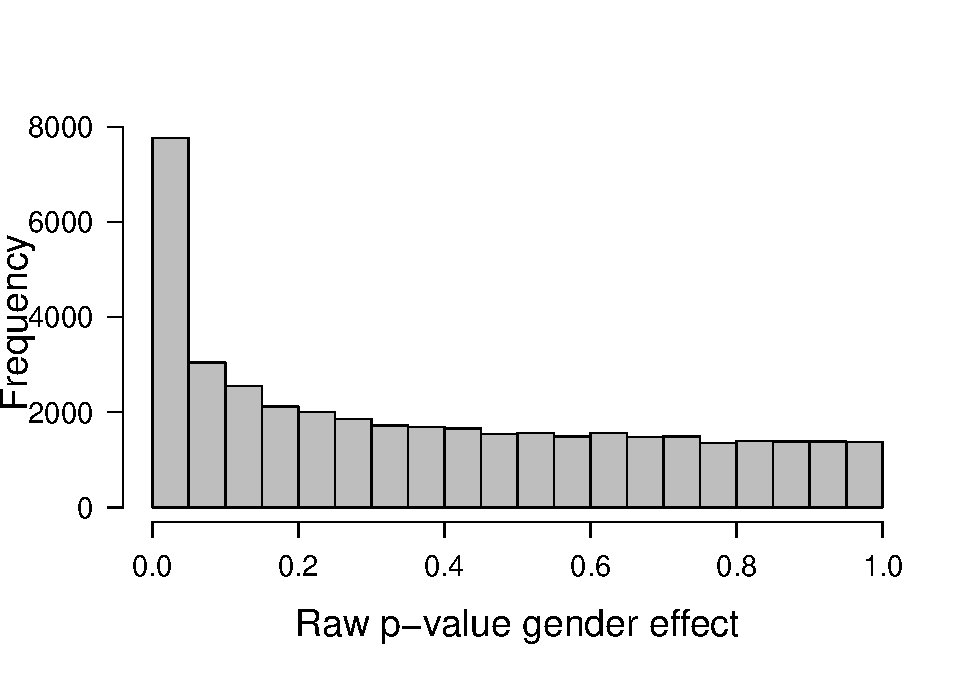
\includegraphics{OmicSHIELD_bookdown_files/figure-latex/plot_hist-1.pdf}

We can also check whether there is inflation just executing

\begin{Shaded}
\begin{Highlighting}[]
\FunctionTok{qqplot}\NormalTok{(ans.gender}\SpecialCharTok{$}\NormalTok{study1}\SpecialCharTok{$}\NormalTok{P.Value)}
\end{Highlighting}
\end{Shaded}

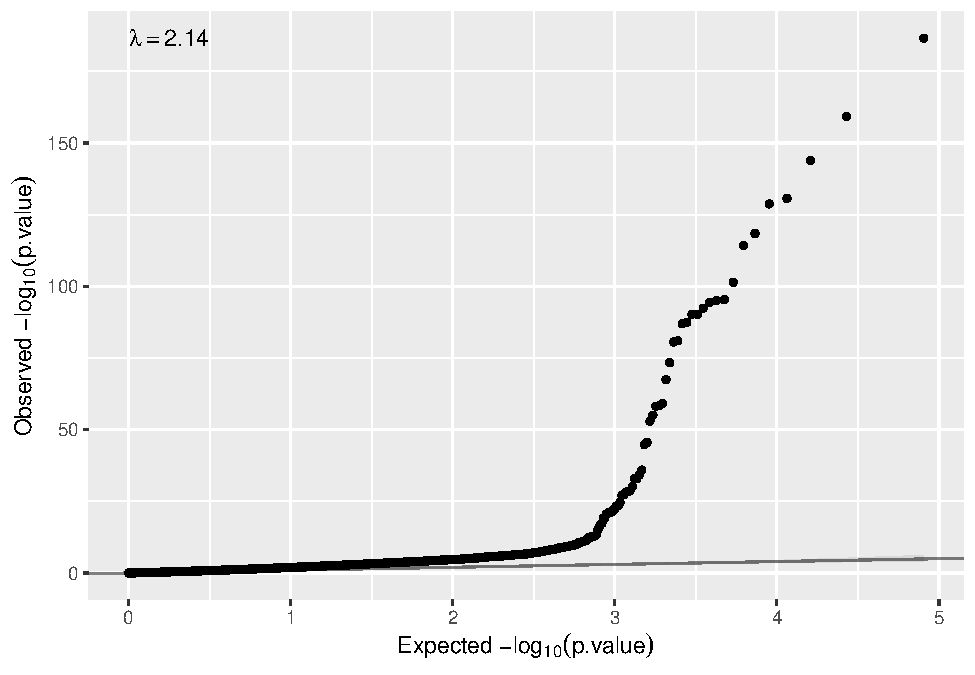
\includegraphics{OmicSHIELD_bookdown_files/figure-latex/plotInfl-1.pdf}

So, in that case, the model needs to remove unwanted variability (\(\lambda>2\)). If so, we can use surrogate variable analysis just changing the argument \texttt{sva=TRUE}

\begin{Shaded}
\begin{Highlighting}[]
\NormalTok{ans.gender.sva }\OtherTok{\textless{}{-}} \FunctionTok{ds.limma}\NormalTok{(}\AttributeTok{model =}  \SpecialCharTok{\textasciitilde{}}\NormalTok{ gdc\_cases.demographic.gender, }
                       \AttributeTok{Set =} \StringTok{"rse.pre"}\NormalTok{, }\AttributeTok{type.data =} \StringTok{"RNAseq"}\NormalTok{,}
                       \AttributeTok{sva =} \ConstantTok{TRUE}\NormalTok{)}
\end{Highlighting}
\end{Shaded}

Now the inflation has dramatically been reduced (\(\lambda>1.12\))

\begin{Shaded}
\begin{Highlighting}[]
\FunctionTok{qqplot}\NormalTok{(ans.gender.sva}\SpecialCharTok{$}\NormalTok{study1}\SpecialCharTok{$}\NormalTok{P.Value)}
\end{Highlighting}
\end{Shaded}

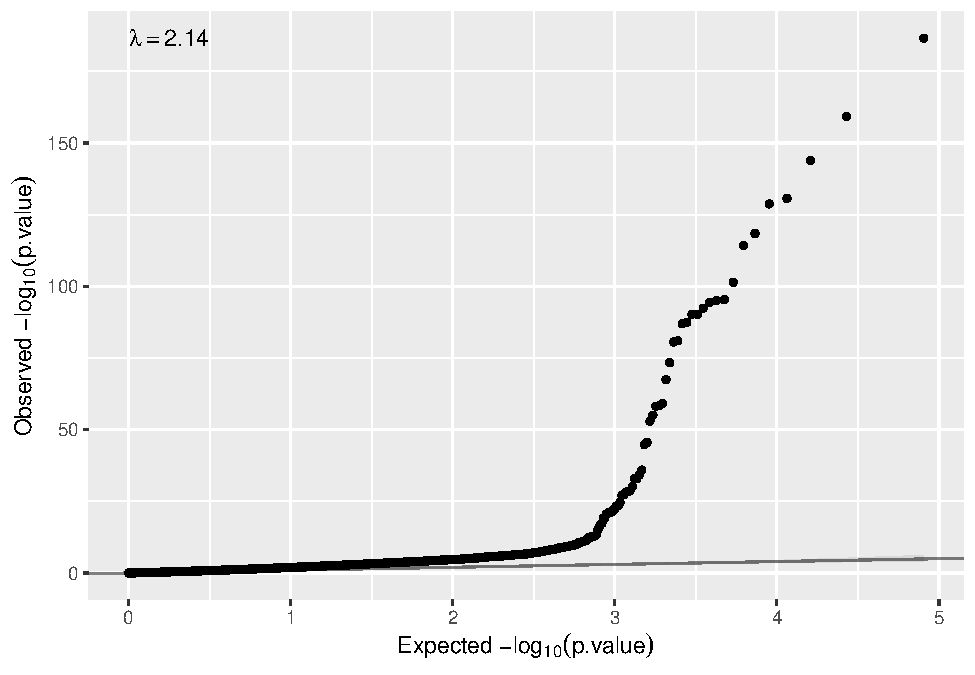
\includegraphics{OmicSHIELD_bookdown_files/figure-latex/plotInfl2-1.pdf}

We can add annotation to the output that is available in our RSE object. We can have access to this information by

\begin{Shaded}
\begin{Highlighting}[]
\FunctionTok{ds.fvarLabels}\NormalTok{(}\StringTok{\textquotesingle{}rse.pre\textquotesingle{}}\NormalTok{)}
\end{Highlighting}
\end{Shaded}

\begin{verbatim}
## $study1
## [1] "chromosome" "start"      "end"        "width"      "strand"    
## [6] "gene_id"    "bp_length"  "symbol"    
## 
## attr(,"class")
## [1] "dsfvarLabels" "list"
\end{verbatim}

So, we can run

\begin{Shaded}
\begin{Highlighting}[]
\NormalTok{ans.gender.sva }\OtherTok{\textless{}{-}} \FunctionTok{ds.limma}\NormalTok{(}\AttributeTok{model =}  \SpecialCharTok{\textasciitilde{}}\NormalTok{ gdc\_cases.demographic.gender, }
                       \AttributeTok{Set =} \StringTok{"rse.pre"}\NormalTok{, }\AttributeTok{type.data =} \StringTok{"RNAseq"}\NormalTok{,}
                       \AttributeTok{sva =} \ConstantTok{TRUE}\NormalTok{, }\AttributeTok{annotCols =} \FunctionTok{c}\NormalTok{(}\StringTok{"chromosome"}\NormalTok{))}
\end{Highlighting}
\end{Shaded}

The results are:

\begin{Shaded}
\begin{Highlighting}[]
\NormalTok{ans.gender.sva}
\end{Highlighting}
\end{Shaded}

\begin{verbatim}
## $study1
## # A tibble: 40,363 x 8
##    id                     n   beta     SE     t   P.Value adj.P.Val chromosome
##    <chr>              <int>  <dbl>  <dbl> <dbl>     <dbl>     <dbl> <chr>     
##  1 ENSG00000274655.1    424 -12.4  0.0761 -52.1 2.74e-187 1.11e-182 chrX      
##  2 ENSG00000270641.1    424 -10.2  0.461  -43.8 5.21e-160 1.05e-155 chrX      
##  3 ENSG00000229807.10   424 -11.0  0.0603 -39.5 1.08e-144 1.45e-140 chrX      
##  4 ENSG00000277577.1    424 -11.3  0.0651 -36.0 2.27e-131 2.29e-127 chrX      
##  5 ENSG00000233070.1    424  10.9  0.0885  35.5 1.85e-129 1.49e-125 chrY      
##  6 ENSG00000260197.1    424  10.2  0.118   32.9 3.72e-119 2.50e-115 chrY      
##  7 ENSG00000213318.4    424  11.4  0.128   31.9 5.57e-115 3.21e-111 chr16     
##  8 ENSG00000278039.1    424  -7.78 0.0812 -28.8 3.85e-102 1.94e- 98 chrX      
##  9 ENSG00000067048.16   424   9.62 0.0894  27.4 4.72e- 96 2.12e- 92 chrY      
## 10 ENSG00000131002.11   424  11.4  0.0924  27.3 9.63e- 96 3.89e- 92 chrY      
## # ... with 40,353 more rows
## 
## attr(,"class")
## [1] "dsLimma" "list"
\end{verbatim}

The function has another arguments that can be used to fit other type of models:

\begin{itemize}
\tightlist
\item
  sva: estimate surrogate variables
\item
  annotCols: to add annotation available in the
\item
  method: Linear regression (``ls'') or robust regression (``robust'') used in limma (\texttt{lmFit})
\item
  robust: robust method used for outlier sample variances used in limma (\texttt{eBayes})
\item
  normalization: normalization method used in the \texttt{voom} transformation (default ``none'')
\item
  voomQualityWeights: should \texttt{voomQualityWeights} function be used instead of \texttt{voom}? (default FALSE)
\item
  big: should SmartSVA be used instead of SVA (useful for big sample size or when analyzing epigenome data. Default FALSE)
\end{itemize}

We have also implemented two other functions \texttt{ds.DESeq2} and \texttt{ds.edgeR} that perform DGE analysis using \href{https://www.bioconductor.org/packages/devel/bioc/vignettes/DESeq2/inst/doc/DESeq2.html}{DESeq2} and \href{https://www.bioconductor.org/packages/release/bioc/vignettes/edgeR/inst/doc/edgeRUsersGuide.pdf}{edgeR} methods. This is the R code used to that purpose:

\textbf{To be supplied}

We close the DataSHIELD session by:

\begin{Shaded}
\begin{Highlighting}[]
\FunctionTok{datashield.logout}\NormalTok{(conns)}
\end{Highlighting}
\end{Shaded}

\hypertarget{epigenome-wide-association-analysis-ewas}{%
\chapter{Epigenome-wide association analysis (EWAS)}\label{epigenome-wide-association-analysis-ewas}}

EWAS requires basically the same statistical methods as those used in DGE. It should be notice that the \textbf{pooled analysis} we are going to illustrate here can also be performed with transcriptomic data since each study must have different range values. If so, gene expression harmonization should be performed, for instance, by standardizing the data at each study. For EWAS where methylation is measured using beta values (e.g CpG data are in the range 0-1) this is not a problem. In any case, adopting the \textbf{meta-analysis} approach could be a safe option.

We have downloaded data from \href{https://www.ncbi.nlm.nih.gov/geo/}{GEO} corresponding to the accesion number GSE66351 which includes DNA methylation profiling (Illumina 450K array) of 190 individuals. Data corresponds to CpGs beta values measured in the superior temporal gyrus and prefrontal cortex brain regions of patients with Alzheimer's. Data have been downloaded using \emph{\href{https://bioconductor.org/packages/3.12/GEOquery}{GEOquery}} package that gets GEO data as \texttt{ExpressionSet} objects. Researchers who are not familiar with \texttt{ExpressionSet}s can read \protect\hyperlink{BioC}{this Section}. Notice that data are encoded as beta-values that ensure data harmonization across studies.

In order to illustrate how to perform data analyses using federated data, we have split the data into two \texttt{ExpressionSet}s having 100 and 90 samples as if they were two different studies. Figure \ref{fig:testResources} shows the two resources defined for both studies (GSE66351\_1 and GSE66351\_2)

In order to perform omic data analyses, we need first to login and assign resources to DataSHIELD. This can be performed using the \texttt{as.resource.object()} function

\begin{Shaded}
\begin{Highlighting}[]
\NormalTok{builder }\OtherTok{\textless{}{-}}\NormalTok{ DSI}\SpecialCharTok{::}\FunctionTok{newDSLoginBuilder}\NormalTok{()}
\NormalTok{builder}\SpecialCharTok{$}\FunctionTok{append}\NormalTok{(}\AttributeTok{server =} \StringTok{"study1"}\NormalTok{, }\AttributeTok{url =} \StringTok{"https://opal{-}demo.obiba.org"}\NormalTok{, }
               \AttributeTok{user =} \StringTok{"dsuser"}\NormalTok{, }\AttributeTok{password =} \StringTok{"P@ssw0rd"}\NormalTok{, }
               \AttributeTok{resource =} \StringTok{"RSRC.GSE66351\_1"}\NormalTok{, }\AttributeTok{profile =} \StringTok{"omics"}\NormalTok{)}
\NormalTok{builder}\SpecialCharTok{$}\FunctionTok{append}\NormalTok{(}\AttributeTok{server =} \StringTok{"study2"}\NormalTok{, }\AttributeTok{url =} \StringTok{"https://opal{-}demo.obiba.org"}\NormalTok{, }
               \AttributeTok{user =} \StringTok{"dsuser"}\NormalTok{, }\AttributeTok{password =} \StringTok{"P@ssw0rd"}\NormalTok{, }
               \AttributeTok{resource =} \StringTok{"RSRC.GSE66351\_2"}\NormalTok{, }\AttributeTok{profile =} \StringTok{"omics"}\NormalTok{)}

\NormalTok{logindata }\OtherTok{\textless{}{-}}\NormalTok{ builder}\SpecialCharTok{$}\FunctionTok{build}\NormalTok{()}

\NormalTok{conns }\OtherTok{\textless{}{-}}\NormalTok{ DSI}\SpecialCharTok{::}\FunctionTok{datashield.login}\NormalTok{(}\AttributeTok{logins =}\NormalTok{ logindata, }\AttributeTok{assign =} \ConstantTok{TRUE}\NormalTok{, }
                               \AttributeTok{symbol =} \StringTok{"res"}\NormalTok{)}
\end{Highlighting}
\end{Shaded}

\begin{verbatim}
## 
## Logging into the collaborating servers
\end{verbatim}

\begin{verbatim}
## 
## Assigning resource data...
\end{verbatim}

\begin{Shaded}
\begin{Highlighting}[]
\CommentTok{\# Assign to the original R class (e.g ExpressionSet)}
\FunctionTok{datashield.assign.expr}\NormalTok{(conns, }\AttributeTok{symbol =} \StringTok{"methy"}\NormalTok{, }
                       \AttributeTok{expr =} \FunctionTok{quote}\NormalTok{(}\FunctionTok{as.resource.object}\NormalTok{(res)))}
\end{Highlighting}
\end{Shaded}

Now, we can see that the resources are actually loaded into the R servers as their original class

\begin{Shaded}
\begin{Highlighting}[]
\FunctionTok{ds.class}\NormalTok{(}\StringTok{"methy"}\NormalTok{)}
\end{Highlighting}
\end{Shaded}

\begin{verbatim}
## $study1
## [1] "ExpressionSet"
## attr(,"package")
## [1] "Biobase"
## 
## $study2
## [1] "ExpressionSet"
## attr(,"package")
## [1] "Biobase"
\end{verbatim}

Then, some Bioconductor-type functions can be use to return non-disclosive information of \texttt{ExpressionSet}s from each server to the client, using similar functions as those defined in the \texttt{dsBaseClient} package. For example, feature names can be returned by

\begin{Shaded}
\begin{Highlighting}[]
\NormalTok{fn }\OtherTok{\textless{}{-}} \FunctionTok{ds.featureNames}\NormalTok{(}\StringTok{"methy"}\NormalTok{)}
\FunctionTok{lapply}\NormalTok{(fn, head)}
\end{Highlighting}
\end{Shaded}

\begin{verbatim}
## $study1
## [1] "cg00000029" "cg00000108" "cg00000109" "cg00000165" "cg00000236"
## [6] "cg00000289"
## 
## $study2
## [1] "cg00000029" "cg00000108" "cg00000109" "cg00000165" "cg00000236"
## [6] "cg00000289"
\end{verbatim}

Experimental phenotypes variables can be obtained by

\begin{Shaded}
\begin{Highlighting}[]
\FunctionTok{ds.varLabels}\NormalTok{(}\StringTok{"methy"}\NormalTok{)}
\end{Highlighting}
\end{Shaded}

\begin{verbatim}
## $study1
##  [1] "title"                   "geo_accession"          
##  [3] "status"                  "submission_date"        
##  [5] "last_update_date"        "type"                   
##  [7] "channel_count"           "source_name_ch1"        
##  [9] "organism_ch1"            "characteristics_ch1"    
## [11] "characteristics_ch1.1"   "characteristics_ch1.2"  
## [13] "characteristics_ch1.3"   "characteristics_ch1.4"  
## [15] "characteristics_ch1.5"   "characteristics_ch1.6"  
## [17] "characteristics_ch1.7"   "characteristics_ch1.8"  
## [19] "molecule_ch1"            "extract_protocol_ch1"   
## [21] "label_ch1"               "label_protocol_ch1"     
## [23] "taxid_ch1"               "hyb_protocol"           
## [25] "scan_protocol"           "description"            
## [27] "data_processing"         "platform_id"            
## [29] "contact_name"            "contact_email"          
## [31] "contact_phone"           "contact_laboratory"     
## [33] "contact_institute"       "contact_address"        
## [35] "contact_city"            "contact_zip/postal_code"
## [37] "contact_country"         "supplementary_file"     
## [39] "supplementary_file.1"    "data_row_count"         
## [41] "age"                     "braak_stage"            
## [43] "brain_region"            "cell type"              
## [45] "diagnosis"               "donor_id"               
## [47] "sentrix_id"              "sentrix_position"       
## [49] "Sex"                    
## 
## $study2
##  [1] "title"                   "geo_accession"          
##  [3] "status"                  "submission_date"        
##  [5] "last_update_date"        "type"                   
##  [7] "channel_count"           "source_name_ch1"        
##  [9] "organism_ch1"            "characteristics_ch1"    
## [11] "characteristics_ch1.1"   "characteristics_ch1.2"  
## [13] "characteristics_ch1.3"   "characteristics_ch1.4"  
## [15] "characteristics_ch1.5"   "characteristics_ch1.6"  
## [17] "characteristics_ch1.7"   "characteristics_ch1.8"  
## [19] "molecule_ch1"            "extract_protocol_ch1"   
## [21] "label_ch1"               "label_protocol_ch1"     
## [23] "taxid_ch1"               "hyb_protocol"           
## [25] "scan_protocol"           "description"            
## [27] "data_processing"         "platform_id"            
## [29] "contact_name"            "contact_email"          
## [31] "contact_phone"           "contact_laboratory"     
## [33] "contact_institute"       "contact_address"        
## [35] "contact_city"            "contact_zip/postal_code"
## [37] "contact_country"         "supplementary_file"     
## [39] "supplementary_file.1"    "data_row_count"         
## [41] "age"                     "braak_stage"            
## [43] "brain_region"            "cell type"              
## [45] "diagnosis"               "donor_id"               
## [47] "sentrix_id"              "sentrix_position"       
## [49] "Sex"                    
## 
## attr(,"class")
## [1] "dsvarLabels" "list"
\end{verbatim}

\hypertarget{single-cpg-analysis}{%
\section{Single CpG analysis}\label{single-cpg-analysis}}

Once the methylation data have been loaded into the opal server, we can perform different type of analyses using functions from the \texttt{dsOmicsClient} package. Let us start by illustrating how to analyze a single CpG from two studies by using an approach that is mathematically equivalent to placing all individual-level.

\begin{Shaded}
\begin{Highlighting}[]
\NormalTok{ans }\OtherTok{\textless{}{-}} \FunctionTok{ds.lmFeature}\NormalTok{(}\AttributeTok{feature =} \StringTok{"cg07363416"}\NormalTok{, }
                    \AttributeTok{model =} \SpecialCharTok{\textasciitilde{}}\NormalTok{ diagnosis }\SpecialCharTok{+}\NormalTok{ Sex, }
                    \AttributeTok{Set =} \StringTok{"methy"}\NormalTok{,}
                    \AttributeTok{datasources =}\NormalTok{ conns)}
\end{Highlighting}
\end{Shaded}

\begin{verbatim}
## Iteration 1...
\end{verbatim}

\begin{verbatim}
## CURRENT DEVIANCE:      7.834782376469
\end{verbatim}

\begin{verbatim}
## Iteration 2...
\end{verbatim}

\begin{verbatim}
## CURRENT DEVIANCE:      5.21465032637778
\end{verbatim}

\begin{verbatim}
## Iteration 3...
\end{verbatim}

\begin{verbatim}
## CURRENT DEVIANCE:      5.21465032637778
\end{verbatim}

\begin{verbatim}
## SUMMARY OF MODEL STATE after iteration 3
\end{verbatim}

\begin{verbatim}
## Current deviance 5.21465032637778 on 187 degrees of freedom
\end{verbatim}

\begin{verbatim}
## Convergence criterion TRUE (0)
\end{verbatim}

\begin{verbatim}
## 
## beta: 0.143108602924252 0.0345988560191347 -0.12176433102489
\end{verbatim}

\begin{verbatim}
## 
## Information matrix overall:
\end{verbatim}

\begin{verbatim}
##               (Intercept) diagnosisCTRL SexM
## (Intercept)           190            84   89
## diagnosisCTRL          84            84   50
## SexM                   89            50   89
\end{verbatim}

\begin{verbatim}
## 
## Score vector overall:
\end{verbatim}

\begin{verbatim}
##                       [,1]
## (Intercept)   1.187939e-13
## diagnosisCTRL 4.898859e-14
## SexM          4.524159e-14
\end{verbatim}

\begin{verbatim}
## 
## Current deviance: 5.21465032637778
\end{verbatim}

\begin{Shaded}
\begin{Highlighting}[]
\NormalTok{ans}
\end{Highlighting}
\end{Shaded}

\begin{verbatim}
##              Estimate Std. Error   p-value
## cg07363416 0.03459886 0.02504291 0.1670998
## attr(,"class")
## [1] "dsLmFeature" "matrix"      "array"
\end{verbatim}

\hypertarget{multiple-cpg-analysis}{%
\section{Multiple CpG analysis}\label{multiple-cpg-analysis}}

The same analysis can be performed for all features (e.g.~CpGs) just avoiding the \texttt{feature} argument. This process can be parallelized using \texttt{mclapply} function from the \texttt{multicore} package.

\begin{Shaded}
\begin{Highlighting}[]
\NormalTok{ans }\OtherTok{\textless{}{-}} \FunctionTok{ds.lmFeature}\NormalTok{(}\AttributeTok{model =} \SpecialCharTok{\textasciitilde{}}\NormalTok{ diagnosis }\SpecialCharTok{+}\NormalTok{ Sex, }
                    \AttributeTok{Set =} \StringTok{"methy"}\NormalTok{,}
                    \AttributeTok{datasources =}\NormalTok{ conns,}
                    \AttributeTok{mc.cores =} \DecValTok{20}\NormalTok{)}
\end{Highlighting}
\end{Shaded}

This method corresponds to the \textbf{pooled analysis} approach and can be very time consiming since the function repeatedly calls the DataSHIELD function \texttt{ds.glm()}. We can adopt another strategy that is to run a glm of each feature independently at each study using \texttt{limma} package (which is really fast) and then combine the results (i.e.~\textbf{meta-analysis} approach).

\begin{Shaded}
\begin{Highlighting}[]
\NormalTok{ans.limma }\OtherTok{\textless{}{-}} \FunctionTok{ds.limma}\NormalTok{(}\AttributeTok{model =} \SpecialCharTok{\textasciitilde{}}\NormalTok{ diagnosis }\SpecialCharTok{+}\NormalTok{ Sex,}
                      \AttributeTok{Set =} \StringTok{"methy"}\NormalTok{, }
                      \AttributeTok{datasources =}\NormalTok{ conns)}
\end{Highlighting}
\end{Shaded}

Then, we can visualize the top genes at each study (i.e server) by

\begin{Shaded}
\begin{Highlighting}[]
\FunctionTok{lapply}\NormalTok{(ans.limma, head)}
\end{Highlighting}
\end{Shaded}

\begin{verbatim}
## $study1
## # A tibble: 6 x 7
##   id             n    beta      SE     t       P.Value adj.P.Val
##   <chr>      <int>   <dbl>   <dbl> <dbl>         <dbl>     <dbl>
## 1 cg13138089   100 -0.147  0.0122  -6.62 0.00000000190  0.000466
## 2 cg23859635   100 -0.0569 0.00520 -6.58 0.00000000232  0.000466
## 3 cg13772815   100 -0.0820 0.0135  -6.50 0.00000000327  0.000466
## 4 cg12706938   100 -0.0519 0.00872 -6.45 0.00000000425  0.000466
## 5 cg24724506   100 -0.0452 0.00775 -6.39 0.00000000547  0.000466
## 6 cg02812891   100 -0.125  0.0163  -6.33 0.00000000731  0.000466
## 
## $study2
## # A tibble: 6 x 7
##   id             n    beta      SE     t      P.Value adj.P.Val
##   <chr>      <int>   <dbl>   <dbl> <dbl>        <dbl>     <dbl>
## 1 cg04046629    90 -0.101  0.0128  -5.91 0.0000000621    0.0172
## 2 cg07664323    90 -0.0431 0.00390 -5.85 0.0000000822    0.0172
## 3 cg27098804    90 -0.0688 0.0147  -5.79 0.000000107     0.0172
## 4 cg08933615    90 -0.0461 0.00791 -5.55 0.000000298     0.0360
## 5 cg18349298    90 -0.0491 0.00848 -5.42 0.000000507     0.0489
## 6 cg02182795    90 -0.0199 0.0155  -5.36 0.000000670     0.0538
\end{verbatim}

The annotation can be added by using the argument \texttt{annotCols}. It should be a vector with the columns of the annotation available in the \texttt{ExpressionSet} or \texttt{RangedSummarizedExperiment} that want to be showed. The columns of the annotation can be obtained by

\begin{Shaded}
\begin{Highlighting}[]
\FunctionTok{ds.fvarLabels}\NormalTok{(}\StringTok{"methy"}\NormalTok{)}
\end{Highlighting}
\end{Shaded}

\begin{verbatim}
## $study1
##  [1] "ID"                          "Name"                       
##  [3] "AddressA_ID"                 "AlleleA_ProbeSeq"           
##  [5] "AddressB_ID"                 "AlleleB_ProbeSeq"           
##  [7] "Infinium_Design_Type"        "Next_Base"                  
##  [9] "Color_Channel"               "Forward_Sequence"           
## [11] "Genome_Build"                "CHR"                        
## [13] "MAPINFO"                     "SourceSeq"                  
## [15] "Chromosome_36"               "Coordinate_36"              
## [17] "Strand"                      "Probe_SNPs"                 
## [19] "Probe_SNPs_10"               "Random_Loci"                
## [21] "Methyl27_Loci"               "UCSC_RefGene_Name"          
## [23] "UCSC_RefGene_Accession"      "UCSC_RefGene_Group"         
## [25] "UCSC_CpG_Islands_Name"       "Relation_to_UCSC_CpG_Island"
## [27] "Phantom"                     "DMR"                        
## [29] "Enhancer"                    "HMM_Island"                 
## [31] "Regulatory_Feature_Name"     "Regulatory_Feature_Group"   
## [33] "DHS"                         "RANGE_START"                
## [35] "RANGE_END"                   "RANGE_GB"                   
## [37] "SPOT_ID"                    
## 
## $study2
##  [1] "ID"                          "Name"                       
##  [3] "AddressA_ID"                 "AlleleA_ProbeSeq"           
##  [5] "AddressB_ID"                 "AlleleB_ProbeSeq"           
##  [7] "Infinium_Design_Type"        "Next_Base"                  
##  [9] "Color_Channel"               "Forward_Sequence"           
## [11] "Genome_Build"                "CHR"                        
## [13] "MAPINFO"                     "SourceSeq"                  
## [15] "Chromosome_36"               "Coordinate_36"              
## [17] "Strand"                      "Probe_SNPs"                 
## [19] "Probe_SNPs_10"               "Random_Loci"                
## [21] "Methyl27_Loci"               "UCSC_RefGene_Name"          
## [23] "UCSC_RefGene_Accession"      "UCSC_RefGene_Group"         
## [25] "UCSC_CpG_Islands_Name"       "Relation_to_UCSC_CpG_Island"
## [27] "Phantom"                     "DMR"                        
## [29] "Enhancer"                    "HMM_Island"                 
## [31] "Regulatory_Feature_Name"     "Regulatory_Feature_Group"   
## [33] "DHS"                         "RANGE_START"                
## [35] "RANGE_END"                   "RANGE_GB"                   
## [37] "SPOT_ID"                    
## 
## attr(,"class")
## [1] "dsfvarLabels" "list"
\end{verbatim}

Then we can run the analysis and obtain the output with the chromosome and gene symbol by:

\begin{Shaded}
\begin{Highlighting}[]
\NormalTok{ans.limma.annot }\OtherTok{\textless{}{-}} \FunctionTok{ds.limma}\NormalTok{(}\AttributeTok{model =} \SpecialCharTok{\textasciitilde{}}\NormalTok{ diagnosis }\SpecialCharTok{+}\NormalTok{ Sex,}
                            \AttributeTok{Set =} \StringTok{"methy"}\NormalTok{, }
                            \AttributeTok{annotCols =} \FunctionTok{c}\NormalTok{(}\StringTok{"CHR"}\NormalTok{, }\StringTok{"UCSC\_RefGene\_Name"}\NormalTok{),}
                            \AttributeTok{datasources =}\NormalTok{ conns)}
\end{Highlighting}
\end{Shaded}

\begin{Shaded}
\begin{Highlighting}[]
\FunctionTok{lapply}\NormalTok{(ans.limma.annot, head)}
\end{Highlighting}
\end{Shaded}

\begin{verbatim}
## $study1
## # A tibble: 6 x 9
##   id          n    beta      SE     t   P.Value adj.P.Val CHR   UCSC_RefGene_Na~
##   <chr>   <int>   <dbl>   <dbl> <dbl>     <dbl>     <dbl> <chr> <chr>           
## 1 cg1313~   100 -0.147  0.0122  -6.62   1.90e-9  0.000466 2     "ECEL1P2"       
## 2 cg2385~   100 -0.0569 0.00520 -6.58   2.32e-9  0.000466 2     "MTA3"          
## 3 cg1377~   100 -0.0820 0.0135  -6.50   3.27e-9  0.000466 17    ""              
## 4 cg1270~   100 -0.0519 0.00872 -6.45   4.25e-9  0.000466 19    "MEX3D"         
## 5 cg2472~   100 -0.0452 0.00775 -6.39   5.47e-9  0.000466 19    "ISOC2;ISOC2;IS~
## 6 cg0281~   100 -0.125  0.0163  -6.33   7.31e-9  0.000466 2     "ECEL1P2"       
## 
## $study2
## # A tibble: 6 x 9
##   id          n    beta      SE     t   P.Value adj.P.Val CHR   UCSC_RefGene_Na~
##   <chr>   <int>   <dbl>   <dbl> <dbl>     <dbl>     <dbl> <chr> <chr>           
## 1 cg0404~    90 -0.101  0.0128  -5.91   6.21e-8    0.0172 11    "CD6"           
## 2 cg0766~    90 -0.0431 0.00390 -5.85   8.22e-8    0.0172 6     "MUC21"         
## 3 cg2709~    90 -0.0688 0.0147  -5.79   1.07e-7    0.0172 11    "CD6"           
## 4 cg0893~    90 -0.0461 0.00791 -5.55   2.98e-7    0.0360 1     ""              
## 5 cg1834~    90 -0.0491 0.00848 -5.42   5.07e-7    0.0489 3     "RARRES1;RARRES~
## 6 cg0218~    90 -0.0199 0.0155  -5.36   6.70e-7    0.0538 8     ""
\end{verbatim}

Then, the last step is to meta-analyze the results. Different methods can be used to this end. We have implemented a method that meta-analyze the p-pvalues of each study as follows:

\begin{Shaded}
\begin{Highlighting}[]
\NormalTok{ans.meta }\OtherTok{\textless{}{-}} \FunctionTok{metaPvalues}\NormalTok{(ans.limma)}
\NormalTok{ans.meta}
\end{Highlighting}
\end{Shaded}

\begin{verbatim}
## # A tibble: 481,868 x 4
##    id                study1      study2   p.meta
##    <chr>              <dbl>       <dbl>    <dbl>
##  1 cg13138089 0.00000000190 0.00000763  4.78e-13
##  2 cg25317941 0.0000000179  0.00000196  1.12e-12
##  3 cg02812891 0.00000000731 0.00000707  1.63e-12
##  4 cg12706938 0.00000000425 0.0000161   2.14e-12
##  5 cg16026647 0.000000101   0.000000797 2.51e-12
##  6 cg12695465 0.00000000985 0.0000144   4.33e-12
##  7 cg21171625 0.000000146   0.00000225  9.78e-12
##  8 cg13772815 0.00000000327 0.000122    1.18e-11
##  9 cg00228891 0.000000166   0.00000283  1.38e-11
## 10 cg21488617 0.0000000186  0.0000299   1.62e-11
## # ... with 481,858 more rows
\end{verbatim}

We can verify that the results are pretty similar to those obtained using pooled analyses. Here we compute the association for two of the top-CpGs:

\begin{Shaded}
\begin{Highlighting}[]
\NormalTok{res1 }\OtherTok{\textless{}{-}} \FunctionTok{ds.lmFeature}\NormalTok{(}\AttributeTok{feature =} \StringTok{"cg13138089"}\NormalTok{, }
                     \AttributeTok{model =} \SpecialCharTok{\textasciitilde{}}\NormalTok{ diagnosis }\SpecialCharTok{+}\NormalTok{ Sex, }
                     \AttributeTok{Set =} \StringTok{"methy"}\NormalTok{,}
                     \AttributeTok{datasources =}\NormalTok{ conns)}
\end{Highlighting}
\end{Shaded}

\begin{verbatim}
## Iteration 1...
\end{verbatim}

\begin{verbatim}
## CURRENT DEVIANCE:      29.765420228408
\end{verbatim}

\begin{verbatim}
## Iteration 2...
\end{verbatim}

\begin{verbatim}
## CURRENT DEVIANCE:      2.43819505985575
\end{verbatim}

\begin{verbatim}
## Iteration 3...
\end{verbatim}

\begin{verbatim}
## CURRENT DEVIANCE:      2.43819505985575
\end{verbatim}

\begin{verbatim}
## SUMMARY OF MODEL STATE after iteration 3
\end{verbatim}

\begin{verbatim}
## Current deviance 2.43819505985575 on 187 degrees of freedom
\end{verbatim}

\begin{verbatim}
## Convergence criterion TRUE (0)
\end{verbatim}

\begin{verbatim}
## 
## beta: 0.443404581787976 -0.137334787076049 -0.0218537351160394
\end{verbatim}

\begin{verbatim}
## 
## Information matrix overall:
\end{verbatim}

\begin{verbatim}
##               (Intercept) diagnosisCTRL SexM
## (Intercept)           190            84   89
## diagnosisCTRL          84            84   50
## SexM                   89            50   89
\end{verbatim}

\begin{verbatim}
## 
## Score vector overall:
\end{verbatim}

\begin{verbatim}
##                        [,1]
## (Intercept)   -9.681145e-14
## diagnosisCTRL -6.980527e-14
## SexM          -5.542788e-14
\end{verbatim}

\begin{verbatim}
## 
## Current deviance: 2.43819505985575
\end{verbatim}

\begin{Shaded}
\begin{Highlighting}[]
\NormalTok{res1}
\end{Highlighting}
\end{Shaded}

\begin{verbatim}
##              Estimate Std. Error      p-value
## cg13138089 -0.1373348 0.01712405 1.057482e-15
## attr(,"class")
## [1] "dsLmFeature" "matrix"      "array"
\end{verbatim}

\begin{Shaded}
\begin{Highlighting}[]
\NormalTok{res2 }\OtherTok{\textless{}{-}} \FunctionTok{ds.lmFeature}\NormalTok{(}\AttributeTok{feature =} \StringTok{"cg13772815"}\NormalTok{, }
                     \AttributeTok{model =} \SpecialCharTok{\textasciitilde{}}\NormalTok{ diagnosis }\SpecialCharTok{+}\NormalTok{ Sex, }
                     \AttributeTok{Set =} \StringTok{"methy"}\NormalTok{,}
                     \AttributeTok{datasources =}\NormalTok{ conns)}
\end{Highlighting}
\end{Shaded}

\begin{verbatim}
## Iteration 1...
\end{verbatim}

\begin{verbatim}
## CURRENT DEVIANCE:      37.4410001835
\end{verbatim}

\begin{verbatim}
## Iteration 2...
\end{verbatim}

\begin{verbatim}
## CURRENT DEVIANCE:      0.692937396766391
\end{verbatim}

\begin{verbatim}
## Iteration 3...
\end{verbatim}

\begin{verbatim}
## CURRENT DEVIANCE:      0.692937396766391
\end{verbatim}

\begin{verbatim}
## SUMMARY OF MODEL STATE after iteration 3
\end{verbatim}

\begin{verbatim}
## Current deviance 0.692937396766391 on 187 degrees of freedom
\end{verbatim}

\begin{verbatim}
## Convergence criterion TRUE (0)
\end{verbatim}

\begin{verbatim}
## 
## beta: 0.471427788697297 -0.0678613723066762 -0.00640757953624292
\end{verbatim}

\begin{verbatim}
## 
## Information matrix overall:
\end{verbatim}

\begin{verbatim}
##               (Intercept) diagnosisCTRL SexM
## (Intercept)           190            84   89
## diagnosisCTRL          84            84   50
## SexM                   89            50   89
\end{verbatim}

\begin{verbatim}
## 
## Score vector overall:
\end{verbatim}

\begin{verbatim}
##                        [,1]
## (Intercept)   -2.370326e-14
## diagnosisCTRL -1.237899e-14
## SexM          -1.260103e-14
\end{verbatim}

\begin{verbatim}
## 
## Current deviance: 0.692937396766391
\end{verbatim}

\begin{Shaded}
\begin{Highlighting}[]
\NormalTok{res2}
\end{Highlighting}
\end{Shaded}

\begin{verbatim}
##               Estimate  Std. Error      p-value
## cg13772815 -0.06786137 0.009128915 1.056225e-13
## attr(,"class")
## [1] "dsLmFeature" "matrix"      "array"
\end{verbatim}

We can create a QQ-plot by using the function \texttt{qqplot} available in our package.

\begin{Shaded}
\begin{Highlighting}[]
\FunctionTok{qqplot}\NormalTok{(ans.meta}\SpecialCharTok{$}\NormalTok{p.meta)}
\end{Highlighting}
\end{Shaded}

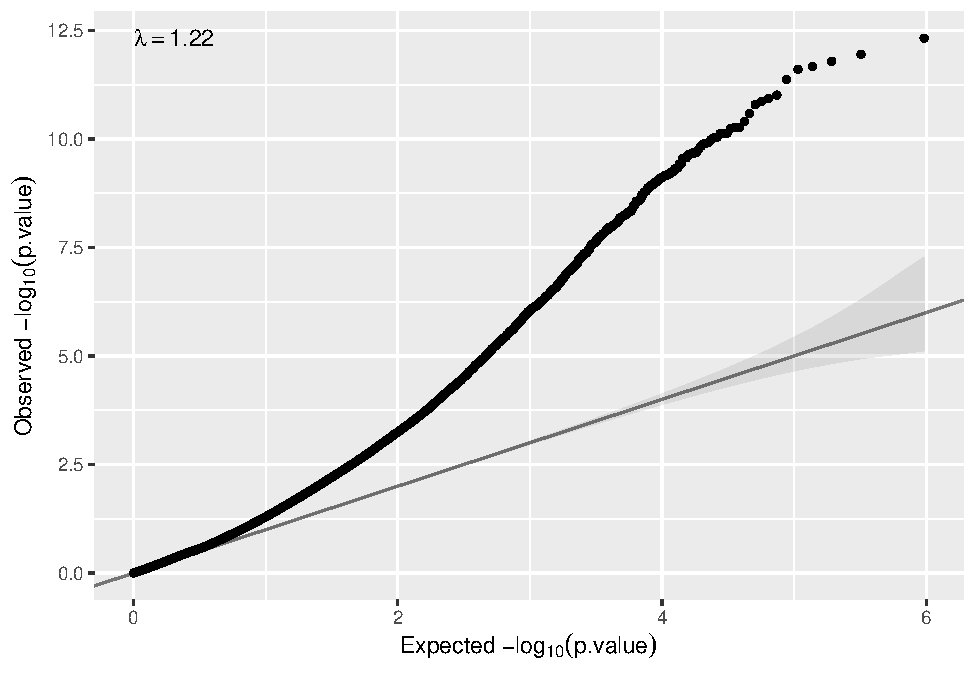
\includegraphics{OmicSHIELD_bookdown_files/figure-latex/qqplot-1.pdf}

Here In some cases inflation can be observed, so that, correction for cell-type or surrogate variables must be performed. We describe how we can do that in the next two sections.

\hypertarget{adjusting-for-surrogate-variables}{%
\section{Adjusting for Surrogate Variables}\label{adjusting-for-surrogate-variables}}

The vast majority of omic studies require to control for unwanted variability. The surrogate variable analysis (SVA) can address this issue by estimating some hidden covariates that capture differences across individuals due to some artifacts such as batch effects or sample quality sam among others. The method is implemented in \emph{\href{https://bioconductor.org/packages/3.12/SVA}{SVA}} package.

Performing this type of analysis using the \texttt{ds.lmFeature} function is not allowed since estimating SVA would require to implement a non-disclosive method that computes SVA from the different servers. This will be a future topic of the \texttt{dsOmicsClient}. NOTE that, estimating SVA separately at each server would not be a good idea since the aim of SVA is to capture differences mainly due to experimental issues among ALL individuals. What we can do instead is to use the \texttt{ds.limma} function to perform the analyses adjusted for SVA at each study.

\begin{verbatim}
## 
## Logging into the collaborating servers
\end{verbatim}

\begin{verbatim}
## 
## Assigning resource data...
\end{verbatim}

\begin{Shaded}
\begin{Highlighting}[]
\NormalTok{ans.sva }\OtherTok{\textless{}{-}} \FunctionTok{ds.limma}\NormalTok{(}\AttributeTok{model =} \SpecialCharTok{\textasciitilde{}}\NormalTok{ diagnosis }\SpecialCharTok{+}\NormalTok{ Sex, }
                    \AttributeTok{Set =} \StringTok{"methy"}\NormalTok{,}
                    \AttributeTok{sva =} \ConstantTok{TRUE}\NormalTok{, }\AttributeTok{annotCols =} \FunctionTok{c}\NormalTok{(}\StringTok{"CHR"}\NormalTok{, }\StringTok{"UCSC\_RefGene\_Name"}\NormalTok{))}
\NormalTok{ans.sva}
\end{Highlighting}
\end{Shaded}

\begin{verbatim}
## $study1
## # A tibble: 481,868 x 9
##    id          n    beta      SE     t  P.Value adj.P.Val CHR   UCSC_RefGene_Na~
##    <chr>   <int>   <dbl>   <dbl> <dbl>    <dbl>     <dbl> <chr> <chr>           
##  1 cg1313~   100 -0.147  0.0122  -6.62  1.90e-9  0.000466 2     "ECEL1P2"       
##  2 cg2385~   100 -0.0569 0.00520 -6.58  2.32e-9  0.000466 2     "MTA3"          
##  3 cg1377~   100 -0.0820 0.0135  -6.50  3.27e-9  0.000466 17    ""              
##  4 cg1270~   100 -0.0519 0.00872 -6.45  4.25e-9  0.000466 19    "MEX3D"         
##  5 cg2472~   100 -0.0452 0.00775 -6.39  5.47e-9  0.000466 19    "ISOC2;ISOC2;IS~
##  6 cg0281~   100 -0.125  0.0163  -6.33  7.31e-9  0.000466 2     "ECEL1P2"       
##  7 cg2766~   100 -0.0588 0.0198  -6.33  7.48e-9  0.000466 16    "ANKRD11"       
##  8 cg1537~   100 -0.0709 0.0115  -6.32  7.83e-9  0.000466 2     "LPIN1"         
##  9 cg1552~   100 -0.0446 0.00750 -6.29  8.69e-9  0.000466 10    ""              
## 10 cg1269~   100 -0.0497 0.00155 -6.27  9.85e-9  0.000475 6     "GCNT2;GCNT2;GC~
## # ... with 481,858 more rows
## 
## $study2
## # A tibble: 481,868 x 9
##    id         n    beta      SE     t P.Value adj.P.Val CHR   UCSC_RefGene_Name 
##    <chr>  <int>   <dbl>   <dbl> <dbl>   <dbl>     <dbl> <chr> <chr>             
##  1 cg040~    90 -0.101  0.0128  -5.91 6.21e-8    0.0172 11    "CD6"             
##  2 cg076~    90 -0.0431 0.00390 -5.85 8.22e-8    0.0172 6     "MUC21"           
##  3 cg270~    90 -0.0688 0.0147  -5.79 1.07e-7    0.0172 11    "CD6"             
##  4 cg089~    90 -0.0461 0.00791 -5.55 2.98e-7    0.0360 1     ""                
##  5 cg183~    90 -0.0491 0.00848 -5.42 5.07e-7    0.0489 3     "RARRES1;RARRES1" 
##  6 cg021~    90 -0.0199 0.0155  -5.36 6.70e-7    0.0538 8     ""                
##  7 cg160~    90 -0.0531 0.0196  -5.31 7.97e-7    0.0548 17    "MEIS3P1"         
##  8 cg012~    90 -0.0537 0.00971 -5.18 1.39e-6    0.0582 7     "HOXA2"           
##  9 cg251~    90 -0.0224 0.00736 -5.15 1.57e-6    0.0582 3     "ZBTB20;ZBTB20;ZB~
## 10 cg074~    90 -0.0475 0.00166 -5.13 1.67e-6    0.0582 22    "C22orf27"        
## # ... with 481,858 more rows
## 
## attr(,"class")
## [1] "dsLimma" "list"
\end{verbatim}

Then, data can be combined meta-anlyzed as follows:

\begin{Shaded}
\begin{Highlighting}[]
\NormalTok{ans.meta.sv }\OtherTok{\textless{}{-}} \FunctionTok{metaPvalues}\NormalTok{(ans.sva)}
\NormalTok{ans.meta.sv}
\end{Highlighting}
\end{Shaded}

\begin{verbatim}
## # A tibble: 481,868 x 4
##    id                study1      study2   p.meta
##    <chr>              <dbl>       <dbl>    <dbl>
##  1 cg13138089 0.00000000190 0.00000763  4.78e-13
##  2 cg25317941 0.0000000179  0.00000196  1.12e-12
##  3 cg02812891 0.00000000731 0.00000707  1.63e-12
##  4 cg12706938 0.00000000425 0.0000161   2.14e-12
##  5 cg16026647 0.000000101   0.000000797 2.51e-12
##  6 cg12695465 0.00000000985 0.0000144   4.33e-12
##  7 cg21171625 0.000000146   0.00000225  9.78e-12
##  8 cg13772815 0.00000000327 0.000122    1.18e-11
##  9 cg00228891 0.000000166   0.00000283  1.38e-11
## 10 cg21488617 0.0000000186  0.0000299   1.62e-11
## # ... with 481,858 more rows
\end{verbatim}

The DataSHIELD session must by closed by:

\begin{Shaded}
\begin{Highlighting}[]
\FunctionTok{datashield.logout}\NormalTok{(conns)}
\end{Highlighting}
\end{Shaded}


  \bibliography{book.bib}

\end{document}
